\documentclass[11pt]{article}
\usepackage[a4paper,margin=2.3cm]{geometry}
\usepackage{graphicx,booktabs,siunitx,amsmath,xcolor}
\usepackage[hidelinks]{hyperref}
\usepackage{caption}
\captionsetup{font=small,labelfont=bf}
\sisetup{detect-all,group-separator={,}}
\graphicspath{{figures/}}
\title{\vspace{-1.2cm}\textbf{Integrating the Atmospheric Water Harvester with the\\
PV-Cleaning Robot: a Coupled Gazebo Simulation and Annual Water--Energy Analysis}}
\author{Autonomous TEC PV-Cleaning Robot --- REE\,598/599}
\date{\today}

\begin{document}
\maketitle
\vspace{-0.6cm}

\begin{abstract}
\noindent The project carried two simulations that never met. One sized a
solar-regenerated silica-gel atmospheric water harvester (AWH) against hourly
climate at six Egyptian sites; the other drove a rail-guided cleaning robot
across a tilted PV panel in Gazebo. This work couples them. A shared dock
reservoir is the bus: each climate day the AWH banks its yield, and each
cleaning pass draws \SI{0.3}{L/m^2} of it. A daily, year-long co-simulation over
the real climate series answers the question the two halves could only assume
separately --- \emph{can the robot harvest the water it needs to clean the array
that powers it?} At residential scale (\SI{9.9}{kWp}, \SI{46}{m^2}) the answer is
yes at every site with a \SIrange{42}{77}{kg} silica bed; the binding constraint
is not the annual average but the worst summer low-humidity spell, which the
arid sites (Benban, Siwa) feel and the humid Delta sites do not. The harvesting
and cleaning together draw \SIrange{1.2}{1.6}{\percent} of the array's own
output while recovering thousands of \si{kWh} a year in avoided soiling loss.
The coupling also runs live in Gazebo: a ROS\,2 water-bus node closes the loop
during a cleaning sweep and reproduces the annual balance to within one cleaning
event.
\end{abstract}

\section{Why integrate the two halves}
The robot needs water and the AWH makes water, but until now those facts lived in
different folders. \texttt{awh\_sim/} produced per-day silica-gel yields for a
\SI{750}{kg} reference bed at six sites, driven by NASA POWER (2020) climate.
\texttt{gazebo/pvbot\_description/} produced a cleaning robot whose spray draws
\SI{0.3}{L/m^2} per pass. Neither knew about the other: the AWH study never saw a
demand, and the robot demo assumed water appeared at the dock. Integration means
making the supply and the demand share one clock and one reservoir, then asking
whether the loop closes --- day by day, site by site, and across the three
deployment scales.

\begin{figure}[ht]\centering
\includegraphics[width=0.78\linewidth]{shot_fill_full.png}
\caption{The integrated Gazebo scene. The resized AWH dock (left, a
\SI{\sim0.4}{m} silica cube on the existing dock plinth, its blue column showing
the live fill level) feeds the rail-guided carriage that sweeps the \SI{24}{\degree}
panel. The tank fill is real geometry; the spray is a visual cue, since Gazebo
Classic carries no fluid solver.}
\end{figure}

\section{The coupling}
\paragraph{Supply.} Two AWH technologies feed the same robot. The primary is the
\emph{solar-regenerated silica gel} of \texttt{awh\_sim}: its annual yield per kg
of gel at each site (\SIrange{25.5}{38.7}{L/kg/yr}, from
\texttt{annual\_summary.csv}) sets the magnitude, and the day-to-day
\emph{shape} from \texttt{annual\_\textit{site}.csv} sets the seasonality. A bed
of mass $m$ then harvests $S_d = m\cdot y_{\text{site}}\cdot s_d$ litres on day
$d$, where $s_d$ is the normalised daily shape ($\sum_d s_d = 1$). The as-built
\emph{thermoelectric (TEC) dock} (\SI{105.97}{g/day} per TEC1-12706 tile at NAC)
is carried as a baseline and a cross-check.

\paragraph{Demand.} Cleaning is triggered by soiling, not a fixed timer. Dust
accrues at \SI{1.0}{\percent/day} of power loss (Benban-class desert) and the
robot cleans when the loss reaches \SI{3.5}{\percent}, which lands the interval
on the design's \SI{3.5}{day} cadence. Each event draws $0.3\cdot A$ litres for
array area $A$.

\paragraph{The reservoir bus.} A dock reservoir of capacity
$\mathrm{cap}=\max(1.5\,E,\,7\,\bar D)$ (one-and-a-half events $E$, or a week of
mean daily demand $\bar D$) buffers the two:
\[
R_d = \mathrm{clip}\!\left(R_{d-1} + S_d - W_d,\; 0,\; \mathrm{cap}\right),
\]
with $W_d=E$ on a cleaning day and $0$ otherwise. A due clean the reservoir
cannot cover is \emph{deferred}: the panel stays dirty, soiling keeps climbing,
and the lost PV energy is booked until the next successful clean. The bed is
sized to $1.20\times$ annual demand; we also solve, by bisection, for the
smallest bed that drives deferrals to zero.

\section{Results}
\subsection{The loop closes at residential scale}
Table~\ref{tab:res} is the headline. Demand is \SI{1435}{L/yr} at every site
(it depends on area and soiling, not climate), and a \SIrange{42}{77}{kg} silica
bed --- a canister that fits the \SI{0.4}{m} dock cube --- covers it everywhere.
The TEC-tile column independently lands on \textbf{38 tiles at NAC}, exactly the
as-built residential dock, which validates the supply model against the
hardware design.

\begin{table}[ht]\centering
\caption{Residential rooftop (\SI{9.9}{kWp}, \SI{46}{m^2}), six Egyptian sites.
$f$ is annual supply\,/\,demand at the sized bed. ``Min kg'' is the bed needed
for zero deferred cleans.}
\label{tab:res}
\small
\begin{tabular}{lcccccc}
\toprule
Site & Demand & Sized bed & Min kg & Deferred & TEC tiles & Parasitic \\
 & (L/yr) & (kg) & (zero-deficit) & cleans & (=demand) & (\% array) \\
\midrule
Benban (Aswan)     & 1435 & 67.6 & 76.5 & 6 & 57 & 1.64 \\
Mansoura           & 1435 & 44.5 & 42.0 & 0 & 38 & 1.32 \\
New Alamein        & 1435 & 46.4 & 42.1 & 0 & 39 & 1.30 \\
Hurghada           & 1435 & 58.0 & 60.9 & 2 & 49 & 1.43 \\
Siwa               & 1435 & 52.0 & 58.2 & 5 & 44 & 1.35 \\
New Admin. Capital & 1435 & 44.6 & 45.5 & 1 & 38 & 1.23 \\
\bottomrule
\end{tabular}
\end{table}

\subsection{The constraint is the summer spell, not the annual average}
The most useful finding only appears once supply and demand share a clock.
Sizing the bed to a \SI{20}{\percent} annual surplus is \emph{not} enough in the
arid sites: Benban still defers 6 cleans, Siwa 5, because a low-humidity summer
stretch (days \(\sim\)120--240) drains the reservoir faster than the bed
refills it (Fig.~\ref{fig:res}, Fig.~\ref{fig:detail}). The humid Delta sites
(Mansoura, New Alamein) ride through with margin to spare --- they need
\emph{less} than the annual sizing. So the bed must be sized to the worst spell,
not the yearly total: Benban needs \SI{76.5}{kg} where its annual figure asks for
\SI{67.6}{kg} (Fig.~\ref{fig:sizing}). This is exactly the kind of conclusion the
two simulations could not reach apart.

\begin{figure}[ht]\centering
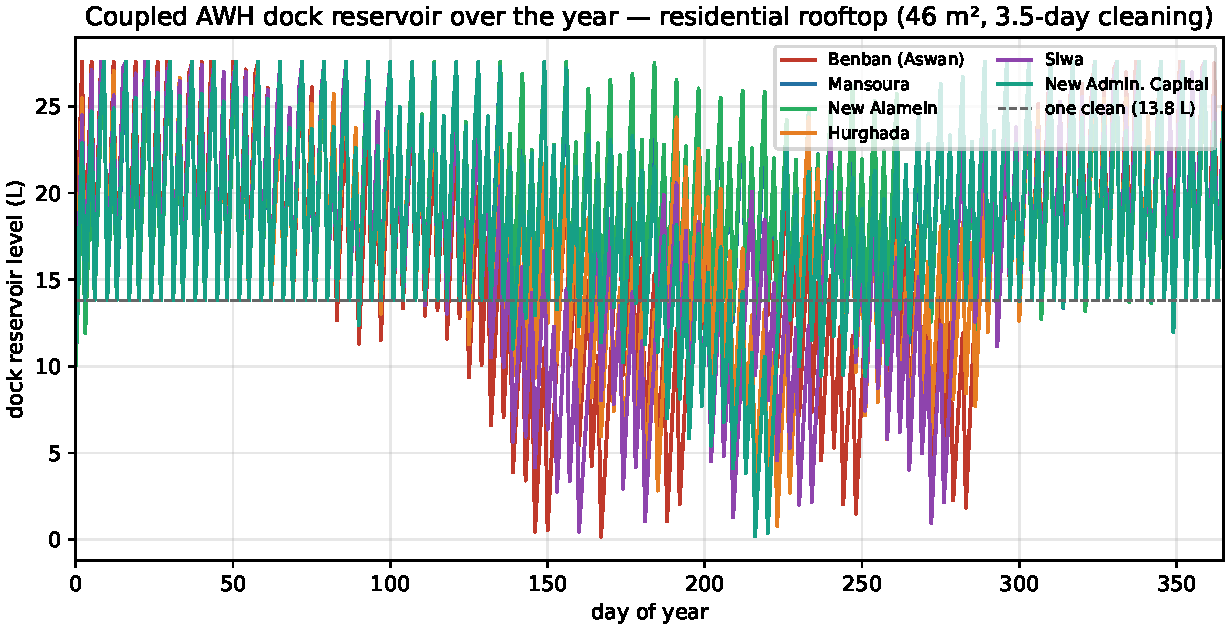
\includegraphics[width=0.86\linewidth]{fig_reservoir_year.pdf}
\caption{Dock reservoir level over the year, six sites, residential scale. The
summer drawdown (days \(\sim\)120--240) pulls the arid sites toward the
one-clean line; the Delta sites stay full.}
\label{fig:res}
\end{figure}

\begin{figure}[ht]\centering
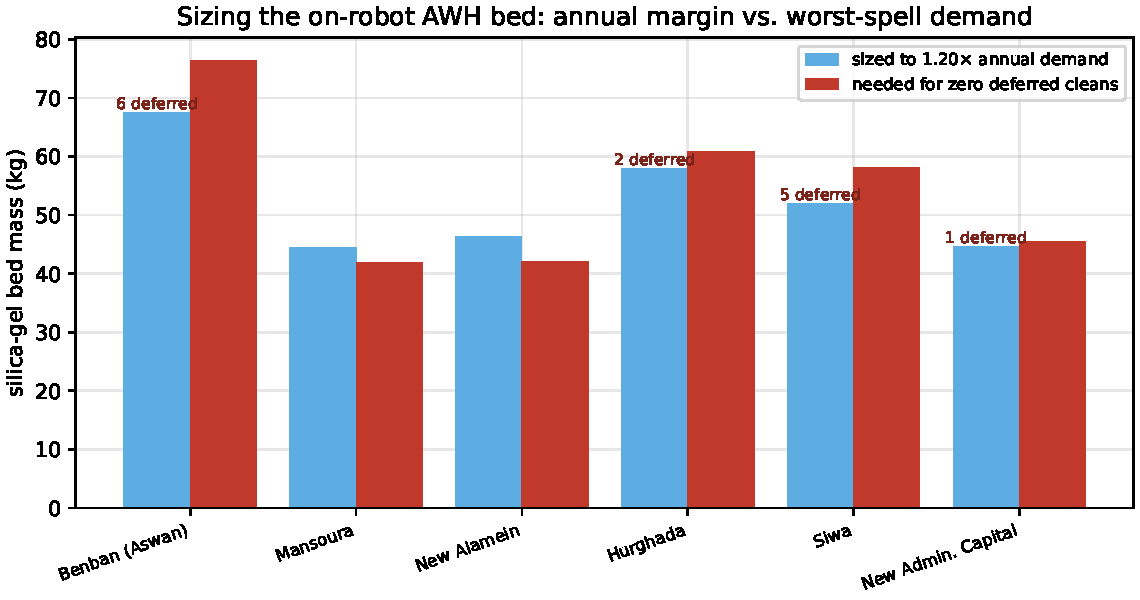
\includegraphics[width=0.70\linewidth]{fig_sizing.pdf}
\caption{Bed sized to the annual margin (blue) vs. the bed needed for zero
deferred cleans (red). Arid sites need more than the annual figure; Delta sites
need less.}
\label{fig:sizing}
\end{figure}

\begin{figure}[ht]\centering
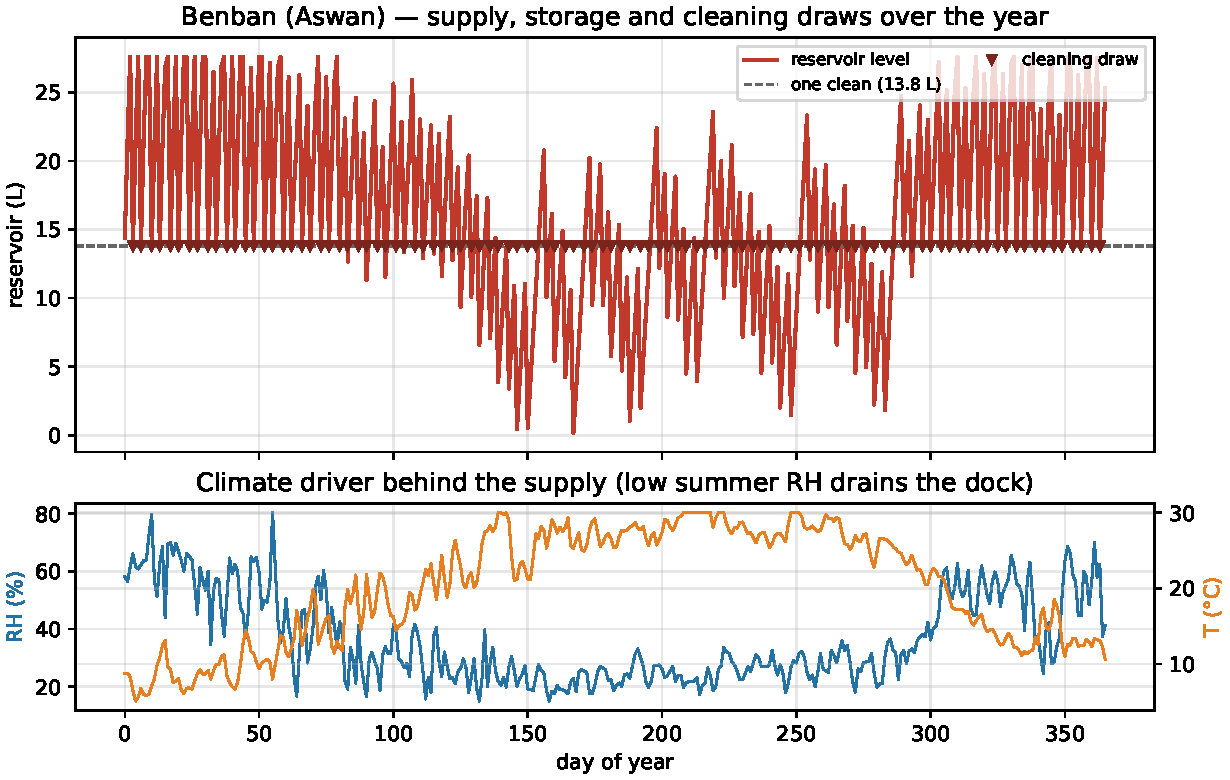
\includegraphics[width=0.80\linewidth]{fig_site_detail.pdf}
\caption{Benban, the hardest site. Top: the reservoir and the cleaning draws
over the year. Bottom: the climate driver --- the summer dip in night relative
humidity is what starves the bed and forces the deferred cleans.}
\label{fig:detail}
\end{figure}

\subsection{Self-supply is scale-invariant; the parasitic load is tiny}
Run at all three scales --- street-lamp (\SI{0.3}{kWp}), residential
(\SI{9.9}{kWp}), commercial (\SI{200}{kWp}) --- the water balance scales
linearly: demand grows with area, the bed grows with it, and the self-supply
fraction is the same curve at every scale (Fig.~\ref{fig:scale}). The commercial
bed lands at \SIrange{0.9}{1.5}{m^3}, matching the ``1\,m$^3$ industrial unit''
of the standalone AWH study; the street-lamp need is 2 tiles, matching the
scaling model. Across all of this the harvesting plus cleaning draws only
\SIrange{1.2}{1.6}{\percent} of the array's own output
(Fig.~\ref{fig:energy}) --- the system pays for itself in energy many times over,
recovering \SIrange{7400}{8900}{kWh/yr} of otherwise-soiled generation at
residential scale (against a never-cleaned panel that saturates near
\SI{50}{\percent} loss).

\begin{figure}[ht]\centering
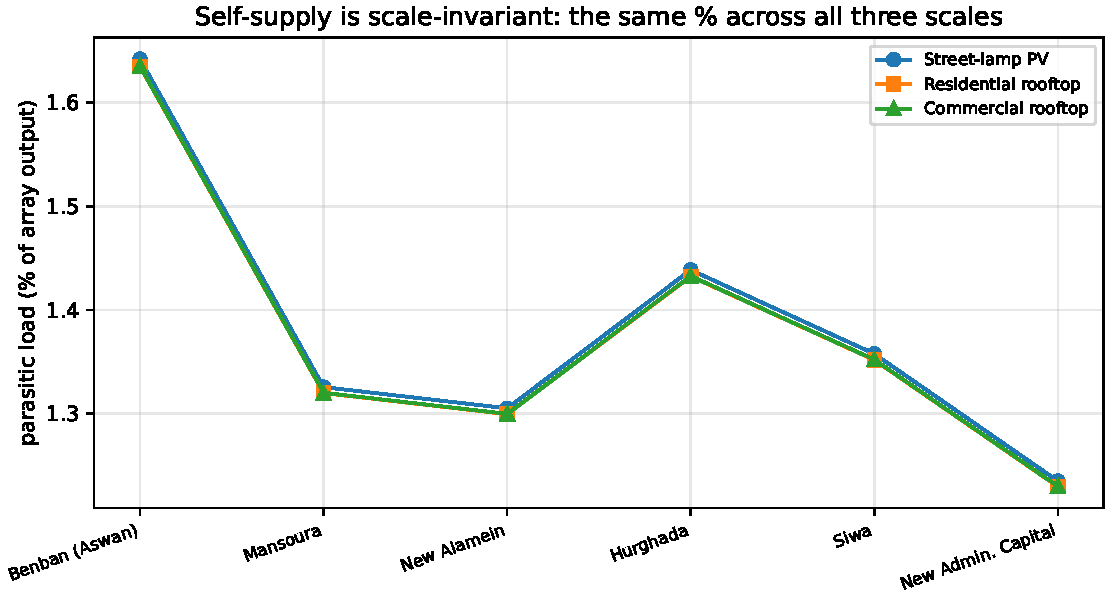
\includegraphics[width=0.62\linewidth]{fig_scale_invariant.pdf}\hfill
\includegraphics[width=0.36\linewidth]{shot_mid_clean.png}
\caption{Left: the parasitic load is the same percentage of array output at all
three scales. Right: a frame from the live coupling --- dock \SI{78}{\percent}
full, panel \SI{48}{\percent} cleaned, \SI{6.7}{L} drawn of a \SI{13.8}{L} event.}
\label{fig:scale}
\end{figure}

\begin{figure}[ht]\centering
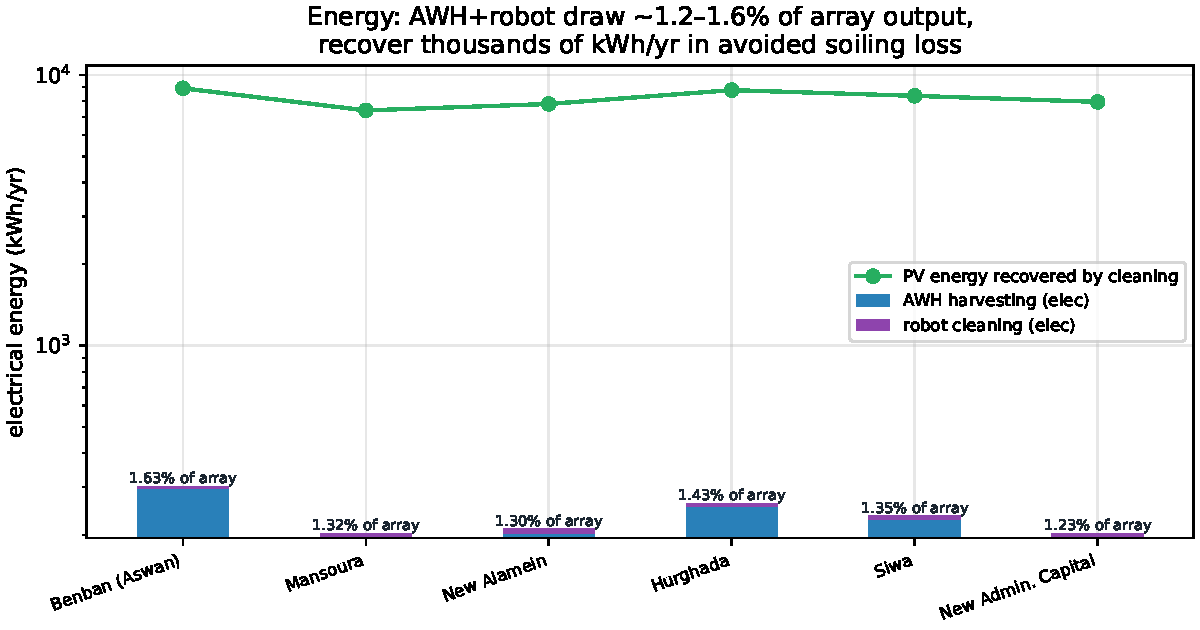
\includegraphics[width=0.80\linewidth]{fig_energy_balance.pdf}
\caption{Electrical energy (log scale): the AWH harvesting and robot cleaning
loads against the PV energy the cleaning recovers. The parasitic fraction is
annotated per site.}
\label{fig:energy}
\end{figure}

\section{The coupling runs live in Gazebo}
The analysis above is a Python co-simulation, but the same loop also runs inside
the ROS\,2 session. \texttt{awh\_water\_bus.py} subscribes to the
\texttt{spray\_on} topic that the coverage driver already publishes during each
cleaning stroke. A compressed clock advances one climate day every few seconds;
each new day the AWH banks its harvest into the dock reservoir, the spray drains
the carriage tank, the dock tops the tank back up between passes, and a running
balance is published on \texttt{/awh/dock\_reservoir} and
\texttt{/awh/self\_supply}. The accounting lives in a plain \texttt{WaterBus}
class with no ROS dependency, so it is unit-tested off-board: driven through a
full year at NAC with a \SI{45}{kg} bed it completes \textbf{101 of \(\sim\)105}
due cleans, harvests \SI{1736}{L} against \SI{1431}{L} sprayed
($f=1.21$, matching the co-sim's \num{1.20}), with a \SI{3.8}{L} deficit --- under
one cleaning event. \texttt{run\_integrated\_demo.sh} brings the whole thing up
in WSL: tilted world with the dock, carriage spawn, cleaning sweep, and the
water bus.

\section{Honest limitations}
\begin{itemize}\setlength\itemsep{1pt}
\item \textbf{No fluid in Gazebo Classic.} The tank fill is real geometry (water
column = reservoir level); the spray is a visual cue. A literal particle stream
is not something this engine produces.
\item \textbf{Soiling is a single linear rate.} \SI{1}{\percent/day} with a
\SI{3.5}{\percent} threshold reproduces the design cadence and is defensible for
desert Egypt, but real soiling is episodic (dust storms, dew, rare rain). The
recovered-energy figure uses a \SI{50}{\percent} saturation cap for a
never-cleaned panel and is therefore an upper bound on the value of cleaning.
\item \textbf{Silica daily shape, summary magnitude.} The per-day column in
\texttt{annual\_\textit{site}.csv} is a single design-point module; the absolute
yield comes from the replicated-module annual summary. We use the column only for
seasonality and the summary for magnitude, which is why the bed sizing is sane
(tens of kg, not tens of tonnes).
\item \textbf{TEC transfer is first-order.} Per-tile yield away from NAC is
scaled by the silica supply ratio, not re-simulated. It is a baseline check, not
a second full model.
\end{itemize}

\section{Reproduce}
\begin{verbatim}
python integration/awh_pvbot_cosim.py     # the coupled annual balance -> results/
python integration/make_figures.py        # all figures -> figures/
python integration/test_water_bus.py      # off-board WaterBus self-check
python integration/build_demo.py          # integrated-world SDFs + demo frames/GIF
bash    integration/run_integrated_demo.sh # live Gazebo+ROS coupling (in WSL)
\end{verbatim}
Outputs: \texttt{results/integration\_sweep.csv} (6 sites $\times$ 3 scales),
\texttt{results/integration\_summary.json}, the six figures, the demo
screenshots and GIF, and the two integrated-world SDFs.

\end{document}
